\documentclass[10pt]{beamer}

\usetheme{metropolis}           % Use metropolis theme

\usepackage{multimedia}
\usepackage{minted}
\usepackage[style=verbose,backend=biber]{biblatex}

\addbibresource{MyReferences.bib}

%% Examples
%
%  \begin{minted}{cpp}
%    class DigitStringDiv1 {
%      public:
%        long long count(string s, int x);
%    };
%  \end{minted}

\title{LED Light Sign \-- ECE 455}

\author{Austin Jones}
\institute{University of Tennessee \-- Knoxville}

\date{\today}

\begin{document}

\maketitle

\begin{frame}{Overview}
  \large
  \tableofcontents
\end{frame}

\section{Background}

\begin{frame}{Roommates and Work-from-Home}
  \Large
  \begin{itemize}
    \item COVID-19 has normalized work from home.
    \item I start a remote job in January.
    \item My roommates love to knock on my door while I'm working.
    \item I am far too susceptible to a long conversation with them.
  \end{itemize}
\end{frame}

\begin{frame}{Solution}
  \begin{figure}
    \centering
    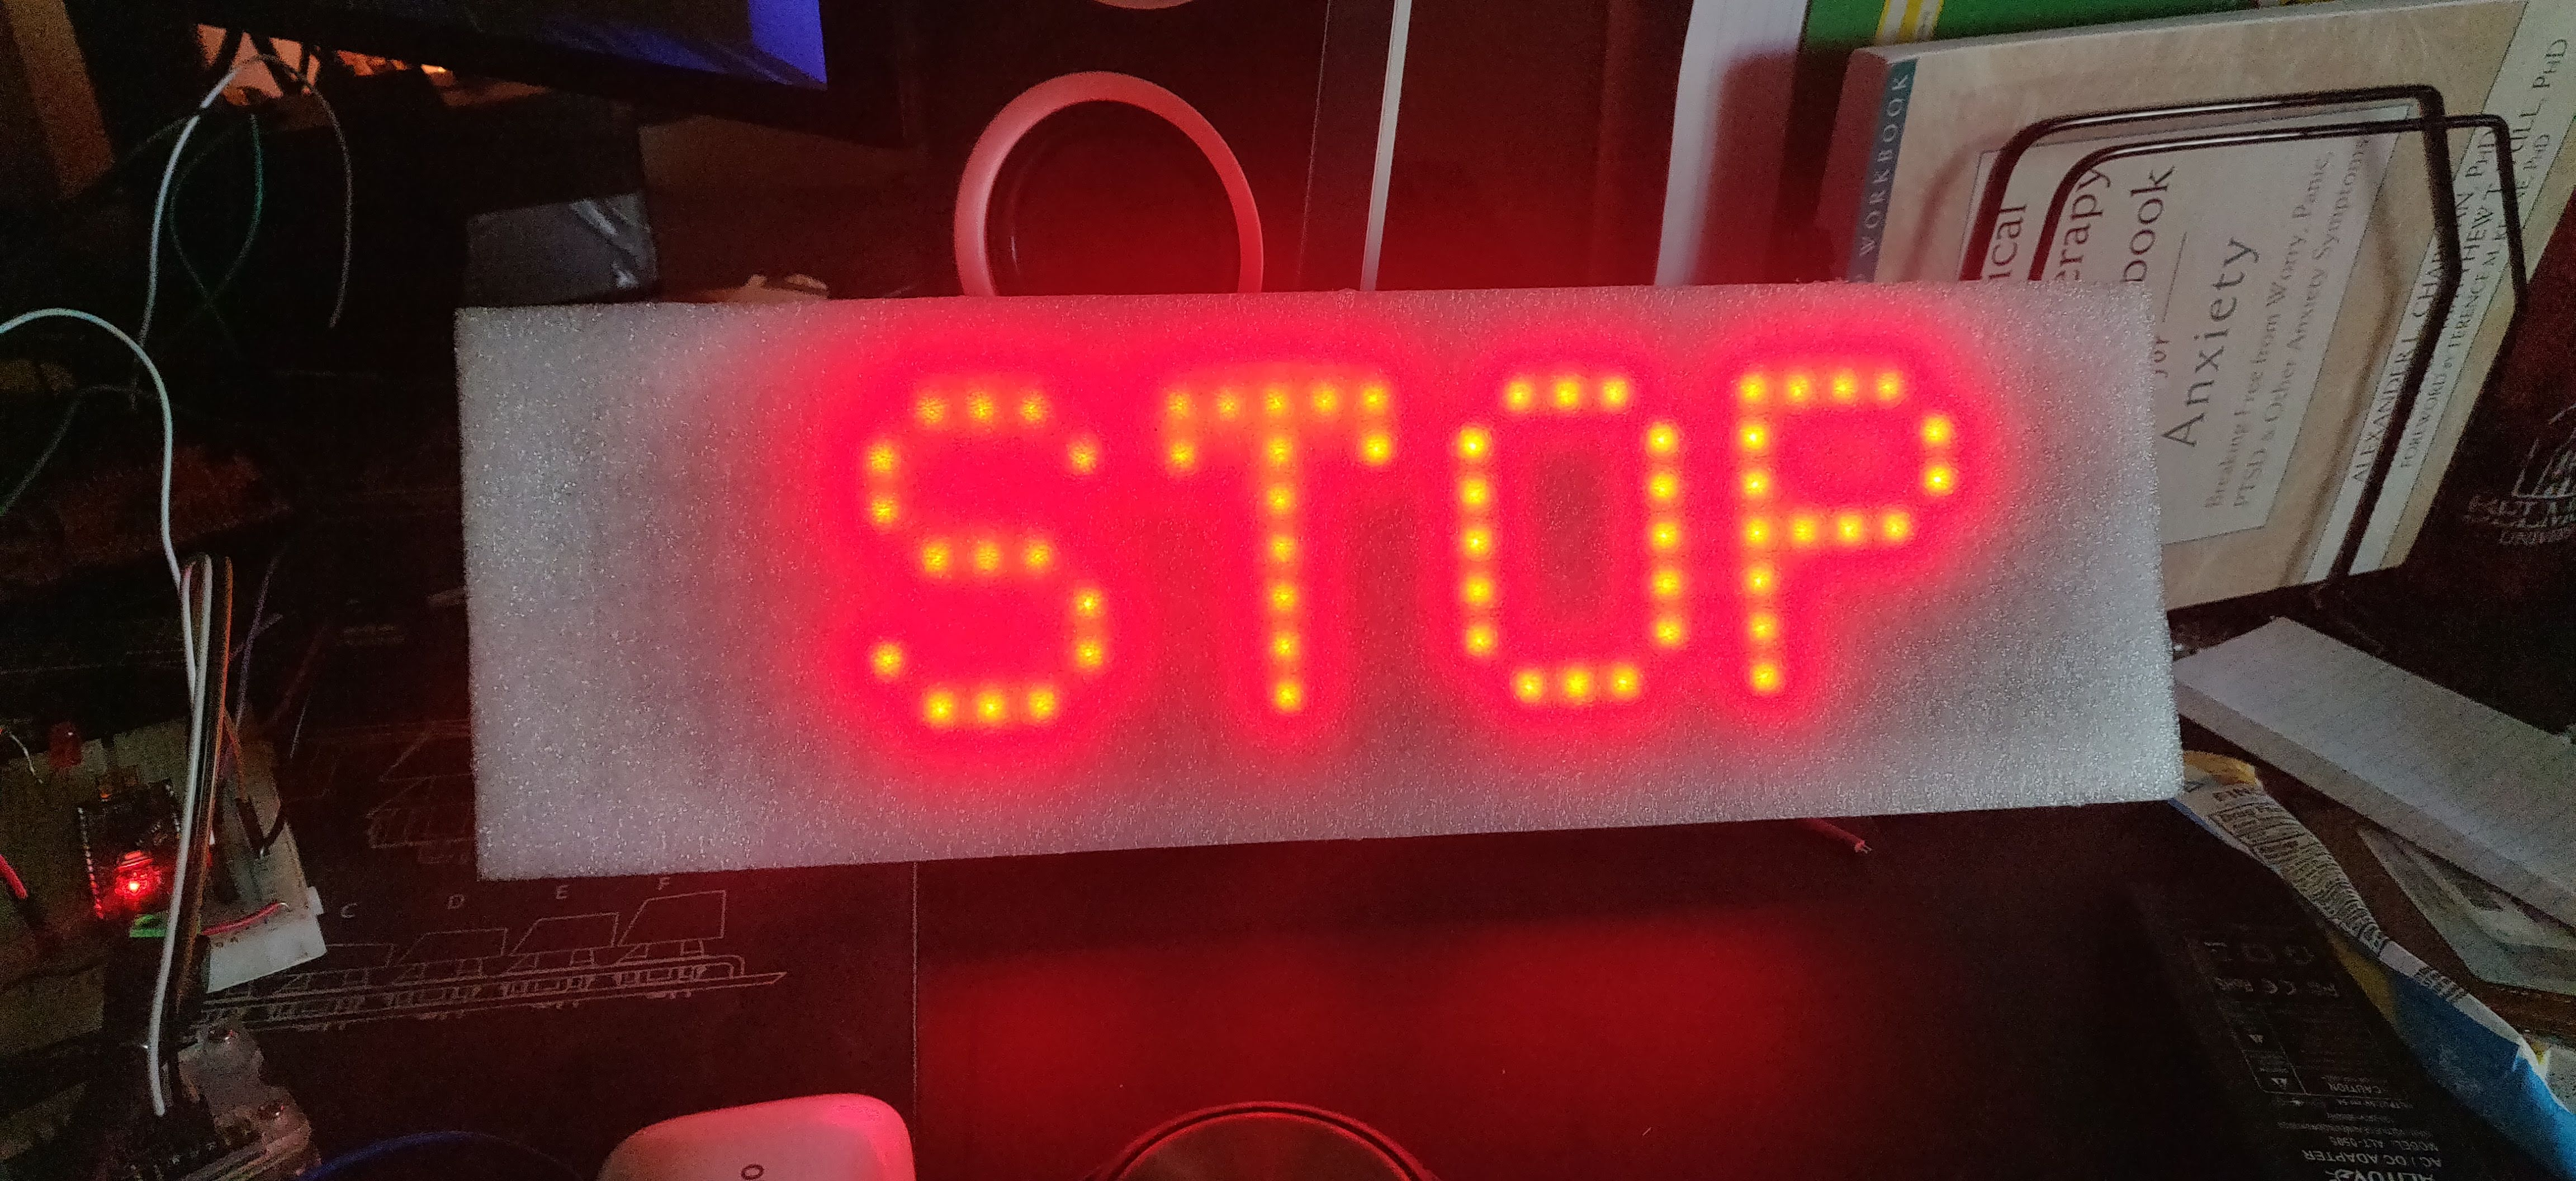
\includegraphics[width=0.8\textwidth]{figures/Stop.jpg}
  \end{figure}
  \centering
  Use an LED Light Sign to display my availability to the outside.
\end{frame}

\begin{frame}{Materials}
  \Large
  \begin{itemize}
    \item Raspberry Pi Zero W
    \item TM4C123 Launchpad\footnote{Arduino Nano used in working implementation}
    \item LED Matrix
    \item Powering solution.
  \end{itemize}
\end{frame}

\section{Existing Solutions}

\begin{frame}{The state of the market}
  \Large
  \begin{itemize}
    \item Use a non-IoT solution: e.g.\ white board, magnet.
      \large
      \begin{itemize}
        \item Can't be automated.
        \item Boring.
      \end{itemize}
    \item Numerous options on Amazon.
      \large
      \begin{itemize}
        \item Expensive: \$150-ish.
        \item Not likely to be live programmable.
        \item The reviews tell bad interfaces.
      \end{itemize}
  \end{itemize}
\end{frame}

\begin{frame}{Why is this worth it?}
  \Large
  \begin{itemize}
    \item Cheaper: \$35
    \item The interface is controllable.
    \item Could be integrated into other smart home solutions.
    \item Proven to be cooler if self-made.
  \end{itemize}
\end{frame}

\section{Methodology}

\begin{frame}{Diagram}
  \begin{figure}
    \centering
    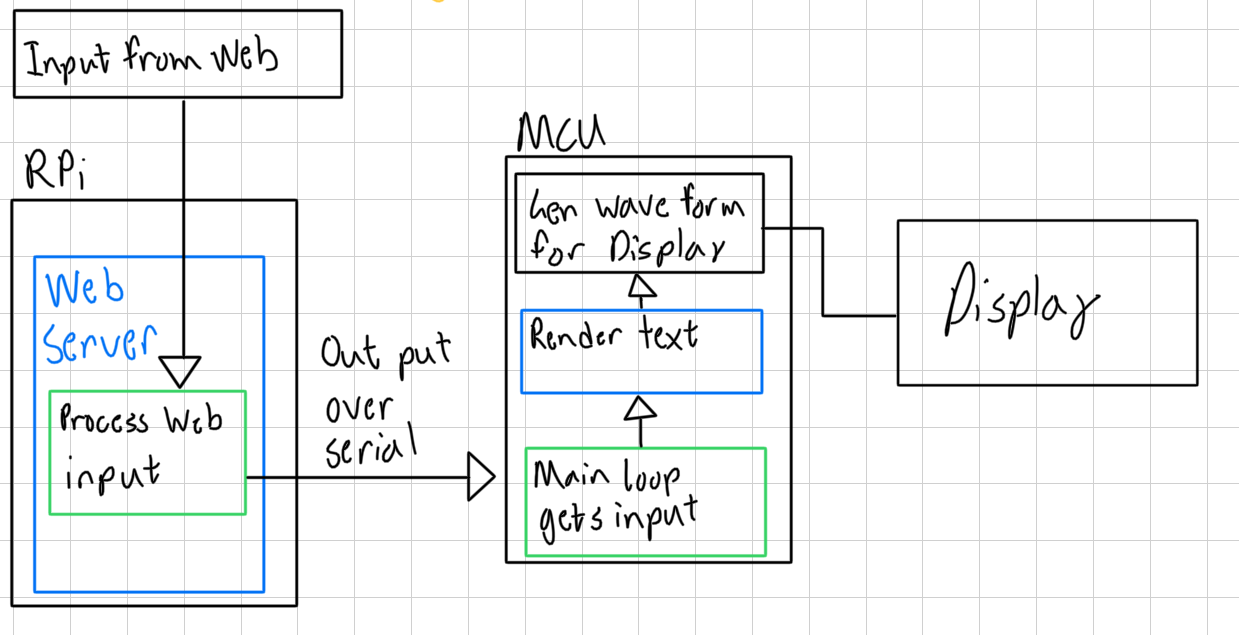
\includegraphics[width=\textwidth]{figures/tot_block_dia.png}
    \caption{Simple Block Diagram for the System}
  \end{figure}
\end{frame}

\begin{frame}{Web Server}
  \large
  Custom web server on Raspberry Pi Zero W
  \begin{itemize}
    \item Written in Rust.
    \item Uses a custom thread pool.
    \item Custom Solution used so the input from the web could be easily piped over an interface.
  \end{itemize}
\end{frame}

\begin{frame}{Light Sign \-- Overview}
  \Large
  \begin{itemize}
    \item Data Stream Description
    \item Rendering Method
  \end{itemize}
\end{frame}
\begin{frame}{Light Sign Data Stream \-- Bits/Packet}
  \begin{columns}
    % Column 1
    \begin{column}{0.7\textwidth}
        \begin{itemize}
          \item Period is set to the time for one bit.
          \item Interrupt on each period.
          \item The duty cycle of the PWM will determine a 1 or 0.
          \item The line is held low for reset.
        \end{itemize}
    \end{column}
    % Column 2
    \begin{column}{0.5\textwidth}
      \begin{figure}
        \centering
        \includegraphics[width=0.7\textwidth]{figures/timing.png}
        \caption{Timing Description}
      \end{figure}
    \end{column}
  \end{columns}
  \begin{figure}
    \centering
    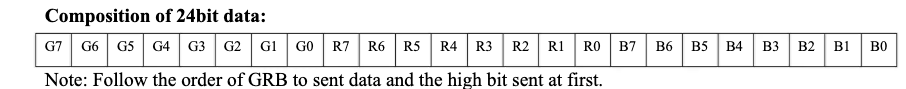
\includegraphics[width=1.0\textwidth]{figures/packet.png}
    \caption{Packet Description}
  \end{figure}
  \footcite{WS2812B}
\end{frame}

\begin{frame}{Light Sign Data Stream\-- Multi-Packet}
  \begin{figure}
    \centering
    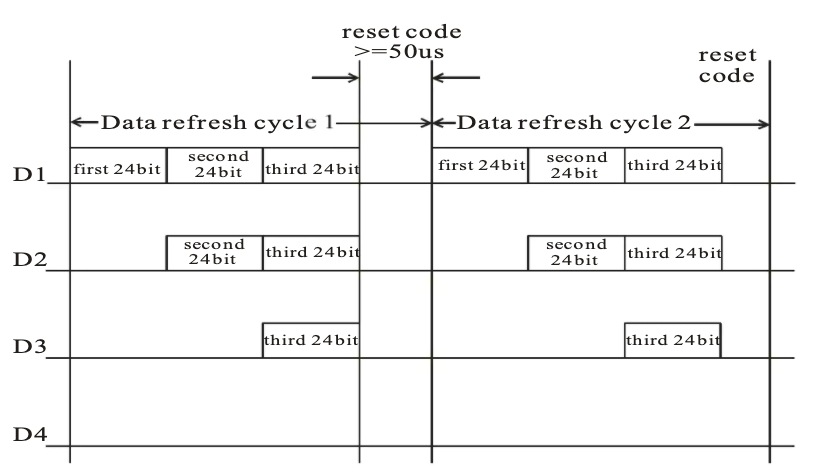
\includegraphics[width=1.0\textwidth]{figures/multi_data.png}
    \caption{Timing for multiple Packets}
  \end{figure}
  \footcite{WS2812B}
\end{frame}

\begin{frame}{Light Sign Rendering}
  \begin{figure}
    \centering
    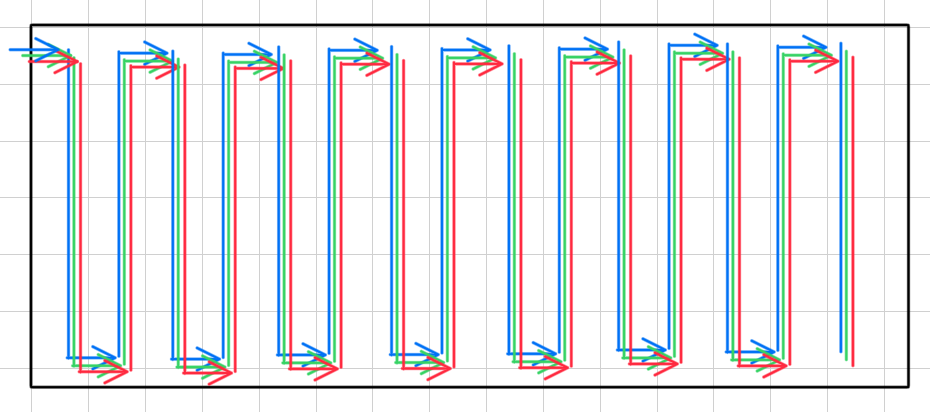
\includegraphics[width=0.8\textwidth]{figures/led_arr.png}
    \caption{LED Arrangement}
  \end{figure}
  \begin{itemize}
    \item Pre-render strings into a serial data stream.
    \item Translate string into indexes into a font header.
    \item Render the strings to the dimensions of the sign.
    \item Flip columns accordingly to appear correct on the screen.
  \end{itemize}
\end{frame}

\section{Results}

\begin{frame}{Overview}
  \Large
  \begin{itemize}
    \item \textbf{Proof of Concept} \-- Works!\\
      RPi 0w + Arduino
    \item \textbf{Tiva MCU + Rust} \-- Doesn't work\\
      RPi 0w + TM4C123 using Rust
    \item \textbf{Tiva MCU + Keil} \-- Doesn't work less\\
      RPi 0w + TM4C123 using C
  \end{itemize}
\end{frame}

\begin{frame}{Proof of Concept}
  \huge Show video of it working. \\ \\
  \small Complain about Beamer and MacOs.
\end{frame}

\begin{frame}{Tiva MCU + Rust}
  \huge Failure\\
  \Large
  \begin{itemize}
    \item Successfully built and flashed the binary.
    \item Via the HAL\@: used basic peripherals.
    \item Cortex-M standard interrupts worked.
    \item \textbf{No other interrupts would work.}
  \end{itemize}
  \huge Show video.
\end{frame}

\begin{frame}{Tiva MCU + Keil}
  \Large
  \begin{itemize}
    \item Could render strings and display the sign.\\
      \large Pre-rendering kept the ISR footprints small.
    \item Some other interrupts could be used in conjunction.
    \item \textbf{The use of UART would ruin the LED sign output.}
  \end{itemize}
  \huge Show video.
\end{frame}

\section{Conclusion}

\begin{frame}{Plans for improvement}
  \Large
  \begin{itemize}
    \item The use of a DMA for the UART could changed the amount it interrupts other ISRs.
    \item A controlled load sequence could also fix this issue.
    \item \textbf{Ultimately, a controller for the light sign would have been the most efficient.}
  \end{itemize}
\end{frame}

\begin{frame}{Plans for Deployment}
  \Large
  \begin{itemize}
    \item PWM dimming for the LED sign.
    \item Solder it into perf-board and make an enclosure.
    \item Add a power switch.
    \item Make the system battery power.
    \item Or clean up cabling.
  \end{itemize}
\end{frame}

\begin{frame}{Thank You}
  \Huge Questions?
\end{frame}

% Add bibliography frame
\begin{frame}{References}
  \printbibliography{}
\end{frame}

\end{document}

